\documentclass[11pt, table, aspectratio=169]{beamer}

%% Note: Beamer is uses' presentation mode' by default (allows for \pause command)
%% adding 'handout' to \document command disables \pause commands
\usepackage[most]{tcolorbox}
\usepackage{xcolor}
\usepackage{listings}
\usepackage{xspace}
\usepackage[export]{adjustbox}
\usepackage{amsmath}
\usepackage{tikz}
\definecolor{codegreen}{rgb}{0,0.6,0}
\definecolor{codegray}{rgb}{0.5,0.5,0.5}
\definecolor{codepurple}{rgb}{0.58,0,0.82}
\definecolor{backcolour}{rgb}{0.95,0.95,0.92}

\newtcolorbox[auto counter,number within=section
]{debox}[1][]{enhanced jigsaw,
	colback=green!0!white,
	coltext={black},
	colframe={black},
	coltitle={black},
	boxrule=0pt,
	frame hidden,
	borderline west={1mm}{0mm}{white!50!red},
	arc=0mm,
	auto outer arc,
	boxsep=5pt,
	left=4pt,
	breakable,
	right=4pt,
	bottom=0pt,
	top=0pt,
	before skip=3mm,
	after skip=3mm,
	%label={def:\thetcbcounter},
	#1}
\PassOptionsToPackage{table,dvipsnames}{xcolor}

%% ----------------------------------------------------------------------------
%% command 'usetheme' searches in directory '../LZSCCslides' for *.sty files 
\makeatletter
\def\beamer@calltheme#1#2#3{%
  \def\beamer@themelist{#2}
  \@for\beamer@themename:=\beamer@themelist\do
  {\usepackage[{#1}]{\beamer@themelocation/#3\beamer@themename}}}

\def\usefolder#1{
  \def\beamer@themelocation{#1}
}
\def\beamer@themelocation{}

\usefolder{LZSCCslides}
\usetheme[]{LUL}
%% ----------------------------------------------------------------------------

%% Site Packages %%
% Required
\usepackage[utf8]{inputenc}  	% Unterstützung für Unicode-Zeichen-Eingabe
\usepackage[T1]{fontenc}      	% Unterstützung für Europäische-Zeichen-Ausgabe
\usepackage{ae}               	% verbesserte Unterstützung für Umlaute  
\usepackage[ngerman]{babel} 	% deutsche Übersetzungen und Wortumbrüche
\usepackage{textcomp}

% Additions
\usepackage{amsmath}            % Erweiterung Mathematisch Umgebung
\usepackage{tabularx}           % Gestaltung Tabellen 
\usepackage{booktabs}           % Gestaltung Tabellen (zusaetzl. Optionen)
\usepackage{hyperref}           % Links

\usepackage{graphicx}           % Einbindung Bilder, Grafiken
\usepackage{epstopdf}           % Einbindung EPS-Bilder
\usepackage{tikz}               % Eigene Erstellung von Grafiken
\usetikzlibrary{positioning}
\usepackage{svg}                % svg-Bilder einbinden

\usepackage{xcolor}             % Verwendung Farben fuer Schrift / Elementen
\usepackage{adjustbox}          % Makros fuer Boxen / Text justierung
\usepackage{tcolorbox}          % Erstellung Boxen (Bspw. fuer Definitionen)
\usepackage{varwidth}           % Umgebung fuer Variable Textbreite (codebox)
\usepackage{setspace}			      % setstretch 

\usepackage{listings}			      % Programm-Code
\usepackage{multicol}           % mehrere Spalten
\usepackage{multirow}           % multirow fuer bessere Tabellen
 
\usepackage{pgfplots}           % HQ Funktion-Plots direkt in TeX erzeugen
\usepgfplotslibrary{dateplot}
\usepackage{xspace}             % Hilfe fuer Leerzeichen nach eigenen Makro-Defintionen

% In order to avoid BigBlueButton problems (converting errors with fonts)
\usepackage{lmodern}

\usepackage{xpatch}


%% Farben =====================================================================
% Unifarben
\definecolor{uniDarkRed}{HTML}{B02F2C}      % granat
\definecolor{uniLightRed}{HTML}{D8413E}     % karneol
\definecolor{uniLightBlue}{HTML}{8AC2D1}    % aquamarin
\definecolor{uniLightGrey}{HTML}{C9C9C9}    % grau (hell)
\definecolor{uniLightBlack}{HTML}{262A31}   % basalt
\definecolor{lightYellow}{HTML}{FFF60C}     % gelb

% Codefarben
\definecolor{pblue}{rgb}{0.13,0.13,1}
\definecolor{pgreen}{rgb}{0,0.5,0}
\definecolor{pred}{rgb}{0.9,0,0}
\definecolor{pgrey}{rgb}{0.46,0.45,0.48}


%% Einstellung Folien =========================================================

% Aufzaehlungen itemize/enumerate (Farbe)
%FORM?
% \setbeamertemplate{itemize items}{\tiny{$\blacksquare$}}
% \setbeamertemplate{itemize subitem}{$\bullet$}

\setbeamercolor{item}{fg=uniDarkRed, bg=uniLightBlack}
\setbeamercolor{subitem}{fg=uniLightRed, bg=uniLightGrey}
\setbeamercolor{subsubitem}{fg=uniLightGrey, bg=uniLightGrey}

% Fussleiste mit aktueller section
\setbeamertemplate{frame footer}{%
  \textcolor{gray}{\thesection\,|\,\textbf{\@currentlabelname}}
}

% Kapitelnummer auf den Section-Seiten, ueberschreibung THEME Einstellung
\setbeamertemplate{section page}{
  \centering
  \begin{tikzpicture}
    [remember picture, overlay]
    \draw node[anchor=south east, align=right] at (0.25,0) (A) {{
        \color{uniLightGrey!90}
        \bfseries
        \fontsize{60pt}{12pt}\selectfont
        \thesection
    }};
    % \node[align=center] at ($(A.north)+(0.0,+0.3)$) {{
    %     \color{uniLightGrey!70}\bfseries\MakeUppercase{Kapitel}
    % }};
  \end{tikzpicture}
  \hspace*{0.3cm}
  \begin{minipage}{22em}
    \raggedright
    \usebeamercolor[fg]{section title}
    \usebeamerfont{section title}
    \insertsectionhead\\[-1ex]
    \usebeamertemplate*{progress bar in section page}
    \par
    \ifx\insertsubsectionhead\@empty\else%
      \usebeamercolor[fg]{subsection title}%
      \usebeamerfont{subsection title}%
      \insertsubsectionhead
    \fi
  \end{minipage}
  \par
  %
}

% Frame title
\setbeamerfont{frametitle}{series=\mdseries}
\AtBeginDocument{\usebeamerfont{normal text}}

% Adjust Table of Contents separation
%\makeatletter
%\patchcmd{\beamer@sectionintoc}{\vskip1.5em}{\vskip0.5em}{}{}
%\makeatother


%% Tikz Settings =========================================================
% Libraries
\usetikzlibrary{calc}
\usetikzlibrary{shapes,arrows}
\usetikzlibrary{decorations.shapes}

% Block styles
\tikzset{
	block1/.style   = {rectangle, draw=uniLightGrey, thick, fill=yellow!20, align=center, rounded corners},
  block2/.style   = {rectangle, draw=black, thick, fill=uniLightBlack!20, align=center, font=\scriptsize\ttfamily},
  line/.style     = {draw, thick, -latex', shorten >=2pt},
  circle1/.style  = {circle,  draw=black, thick, align=center, font=\footnotesize\ttfamily},
  decide1/.style  = {diamond,  draw=black, thick, fill=yellow!20, align=center, font=\footnotesize\ttfamily}
}


%% User-defined Commands / Environments ==============================================
% Einrueckungen
\newcommand{\boxskip}{\hspace*{7pt}}   
\newcommand{\itemskip}{\hspace*{13pt}} % align listings mit itemize Umgebung
\newcommand{\codeskip}{\hspace*{35pt}} % align listings mit 1. Ebene Anfuehrung (mit ZEICHEN)

% Text
\newcommand{\textcode}[2]{{\ttfamily\color{#1} #2}}
\newcommand{\dbl}[0]{\textquotedbl}
\newcolumntype{C}[1]{>{\centering}p{#1}}

% Codeboxes -----------------------------------------------
%kleine Box
\newcommand{\smallcodebox}[1]{ %
  \fcolorbox{uniLightGrey!80}{white}{{\footnotesize\ttfamily #1}}\vspace*{2pt}
}

%BIg Box
%DOES NOT WORK WITH \textcode (COLOR) (?) -> use \textcolor 
%end text with \par, to avoid irregular line separation
%optional: define color for box, e.g. \simplebox[pblue]{...}
\newcommand{\simplebox}[2][black]{%
  \vspace*{2pt}
  \begin{tcolorbox}%
    [hbox, size=small,  nobeforeafter,colback=white, %
    colframe=uniLightGrey!80, boxrule = 1pt, shrink tight, %
    sharp corners, boxsep = 5pt, left=0pt]
    \color{#1}
    \begin{varwidth}{\textwidth}
      {\footnotesize\ttfamily\setstretch{1.0}
          #2
          \par
      }
    \end{varwidth}
  \end{tcolorbox}
  \vspace*{-2pt}
}


%% Code Style =================================================================
\lstdefinestyle{basic}{
  basicstyle=\ttfamily\scriptsize,
  commentstyle=\color{pgreen},
  keywordstyle=\color{pblue},
  stringstyle=\color{pred},
  moredelim=[il][\textcolor{pgrey}],
  backgroundcolor=\color{uniLightGrey!30},
  numbers=left,
  numberstyle=\tiny\color{pgrey!80},
  framexleftmargin=1em,
  tabsize=2,
  showtabs=false,
  showspaces=false,                
  showstringspaces=false,
  breaklines=true
}



%% Backup =====================================================================
%\newcommand{\backupbegin}{
%   \newcounter{framenumberappendix}
%   \setcounter{framenumberappendix}{\value{framenumber}}
%}
%\newcommand{\backupend}{
%   \addtocounter{framenumberappendix}{-\value{framenumber}}
%   \addtocounter{framenumber}{\value{framenumberappendix}} 
%}

\newenvironment<>{varblock}[2][.9\textwidth]{%
  \setlength{\textwidth}{#1}
  \begin{actionenv}#3%
    \def\insertblocktitle{#2}%
    \par%
    \usebeamertemplate{block begin}
}{\par%
    \usebeamertemplate{block end}%
  \end{actionenv}
}


\linespread{1.05} % manual set one-half spacing

\xpatchcmd{\itemize}
{\def\makelabel}
{\ifnum\@itemdepth=1\relax
    \setlength\itemsep{2ex}% separation for first level
\else
    \ifnum\@itemdepth=2\relax
    \setlength\itemsep{1ex}% separation for second level
    \else
    \ifnum\@itemdepth=3\relax
        \setlength\itemsep{0.75ex}% separation for third level
\fi\fi\fi\def\makelabel
}
{}
{}


\subtitle{LZMSCI521M}
\date{\today}
%\date{}
\author{Dr Nono Saha}
\institute{University of Leipzig/ ScaDS.AI}
\def\week{1}



\newcommand{\gd}[2]{\begin{debox}[label=#1]#2\end{debox}}


\begin{document}
	
	\setcounter{framenumber}{0}
	\setcounter{section}{0}
	
	\title{VMA Translation in Multi-process OS}
	
	\maketitle
	%
	
	
	\begin{frame}{What Will You Learn Today?}
		%\scriptsize
		\setbeamertemplate{section in toc}[sections numbered]
		\tableofcontents[hideallsubsections]
		%\thispagestyle{empty}
	\end{frame}
	\title{Micro-Course: Virtual Memory Address Translation in Multi-process OS}
	\author{For Second-year Computer Science Students}
	\date{}
	
	\section{\textbf{Virtual Memory}}

\begin{frame}{Why Virtual Memory?}
	\begin{figure}
		\centering
		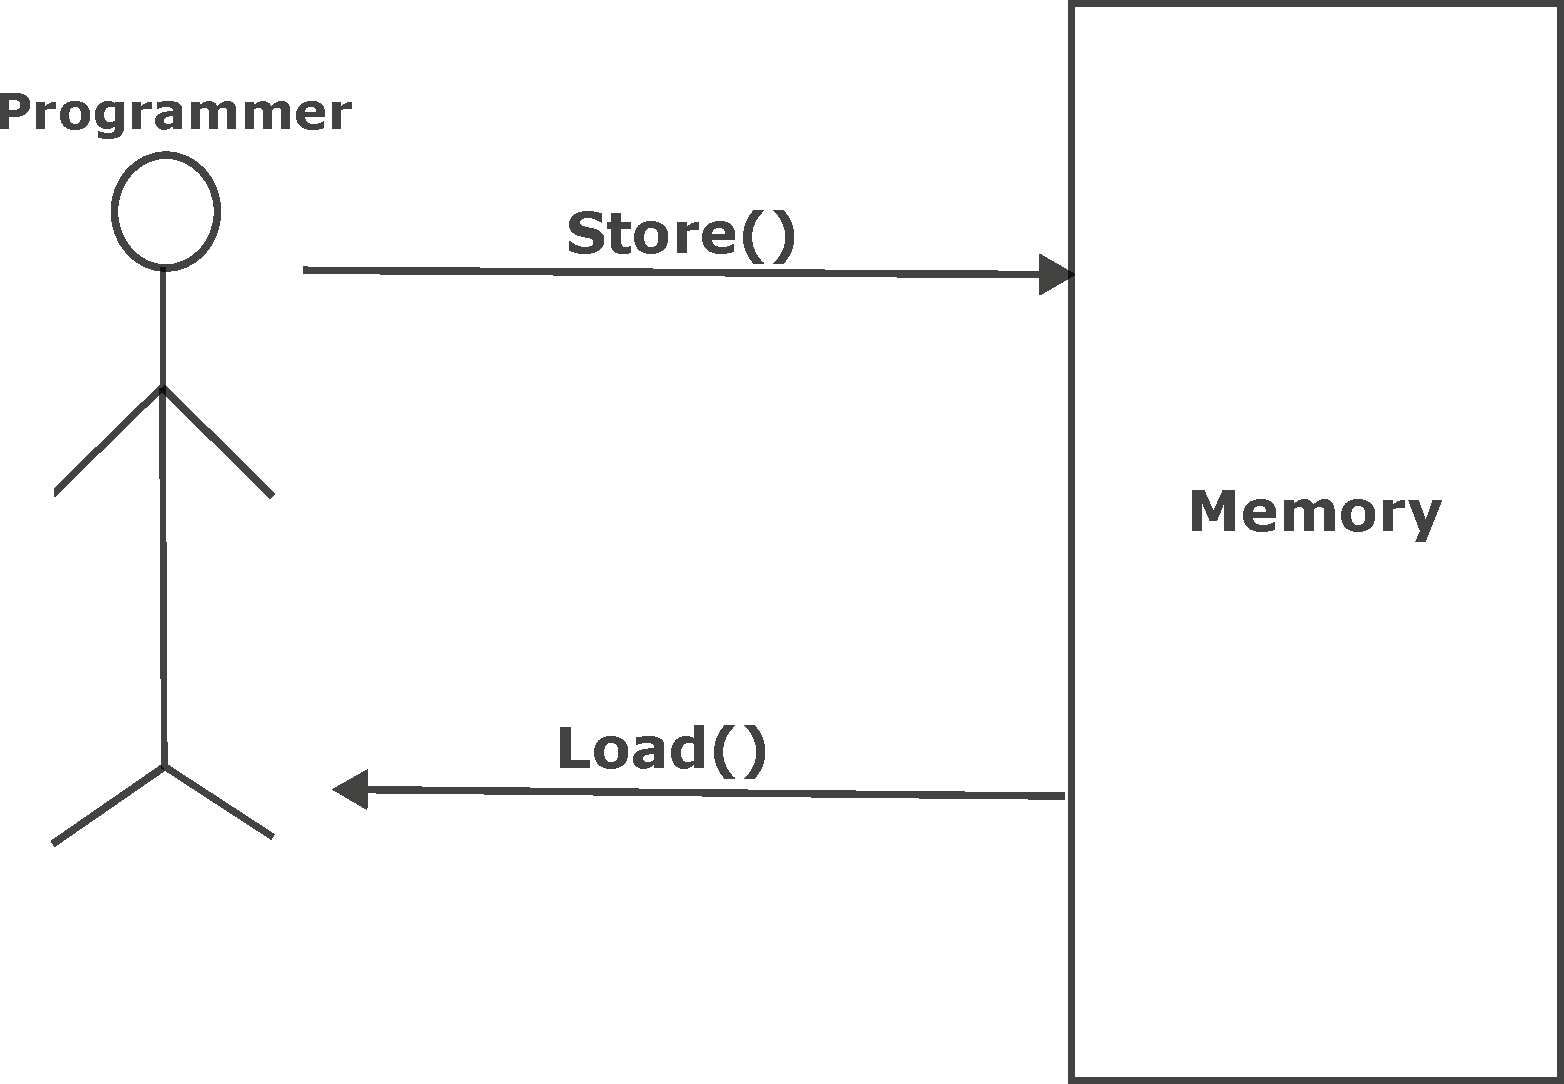
\includegraphics[width=0.5 \linewidth ]{pic/memory2.pdf}
	\end{figure}
	\vspace{-0.45cm}
	\textbf{Possible problems}
	\begin{enumerate}
		\item Computers have limited physical memory, but modern programs expect a large address space.
		\item Different programs (processes) need to be isolated: can't let one process overwrite another's memory!
		\item The ISA often supports a larger address space than there is physical memory.
	\end{enumerate}
\end{frame}

		\begin{frame}[fragile]{\textbf{Virtual Memory Concepts}}
%Imagine you and a friend are both typing essays on separate computers, both saving to a file called \texttt{essay.docx}. There's no danger of overwriting each other's file because each computer provides a private workspace. Similarly, \textbf{virtual memory} gives each process its own private address space.
\begin{itemize}
			\item \textbf{Idea}: Give the programmer the illusion of a large addressspace while having a small physical memory. 
			\begin{itemize}
				\item So that the programmer does not worry about managing physical memory.
			\end{itemize}
			
			\item Programmer can assume having an ``infinite'' amount of physical memory
			
			
			\item Hardware and software cooperatively and automatically manage the physical memory space to provide the illusion
			 
			 \begin{itemize}
			 	\item Illusion is maintained for each independent process
			 \end{itemize}
		
		\end{itemize}
			 
			\textbf{Example:} Suppose a process wants to read byte \texttt{0x2400} (virtual).		
			\vspace{-0.4cm}
			\begin{center}
				\begin{tikzpicture}
					% Virtual Memory
					\draw[fill=blue!10] (-3,2) rectangle (1,3);
					\node at (-1,2.5) {\texttt{VM 0x2000-0x2FFF}};
					% Arrow to Page Table
					\draw[->, thick] (1,2.5) -- (2,2.5);
					% Page Table
					\draw[fill=green!10] (2,2) rectangle (6,3.2);
					\node at (4,2.9) {Translator (Page Table):};
					\node[anchor=west] at (1.9,2.4) {Page 2 $\rightarrow$ Frame 5};
					% Arrow to Physical Memory
					\draw[->, thick] (6,2.5) -- (7,2.5);
					% Physical Memory
					\draw[fill=red!10] (7,2) rectangle (11,3);
					\node at (9,2.5) {\texttt{RAM 0x5000-0x5FFF}};
				\end{tikzpicture}
			\end{center}
			Thus, virtual address \texttt{0x2400} maps to physical address \texttt{0x5400}.
			
		\end{frame}
		
		\begin{frame}[fragile]{\textbf{Example of Translation in Multi-Process Situation}}

		\textbf{Process A:} Virtual \texttt{0x4000 (Page 4)} $\rightarrow$ Frame 12 $\rightarrow$ \texttt{0xC000}

\textbf{Process B:} Virtual \texttt{0x4000 (Page 4)} $\rightarrow$ Frame 7 $\rightarrow$ \texttt{0x7000}

\begin{center}
	\begin{tikzpicture}
		% Process A
		\draw[fill=blue!10] (0,2) rectangle (2,2.8);
		\node at (1,2.4) {\texttt{A: 0x4000}};
		\draw[->, thick] (2,2.4) -- (4,2.4);
		\draw[fill=red!10] (6,2.) rectangle (4,2.8);
		\node at (5,2.4) {\texttt{0xC000}};
		% Process B
		\draw[fill=green!10] (0,0.8) rectangle (2,1.6);
		\node at (1,1.2) {\texttt{B: 0x4000}};
		\draw[->, thick] (2,1.2) -- (4,1.2);
		\draw[fill=red!10] (4,0.8) rectangle (6,1.7);
		\node at (5,1.2) {\texttt{0x7000}};
	\end{tikzpicture}
\end{center}

Both processes use the same virtual address but access different physical locations.
		\end{frame}
		
\begin{frame}[fragile]{\textbf{Basic Mechanism}}
	\begin{itemize}
		\item Indirection (in addressing) 
		\item Address generated by each instruction in a program is a ``virtual address'' 
		
		\begin{itemize}
			\item  i.e., it is not the physical address used to address main memory
			\item   called ``linear address'' in \texttt{x86}
			
		\end{itemize}
		\item An ``address translation'' mechanism maps this address to a ``physical address''
		\begin{itemize}
			\item called ``real address'' in \texttt{x86q} 
			\item Address translation mechanism can be implemented in hardware and software together 
		\end{itemize}
		 
	\end{itemize}
\end{frame}
		

\begin{frame}{\textbf{A system with Virtual Memory (Page based)}}
	\begin{figure}
		\centering
		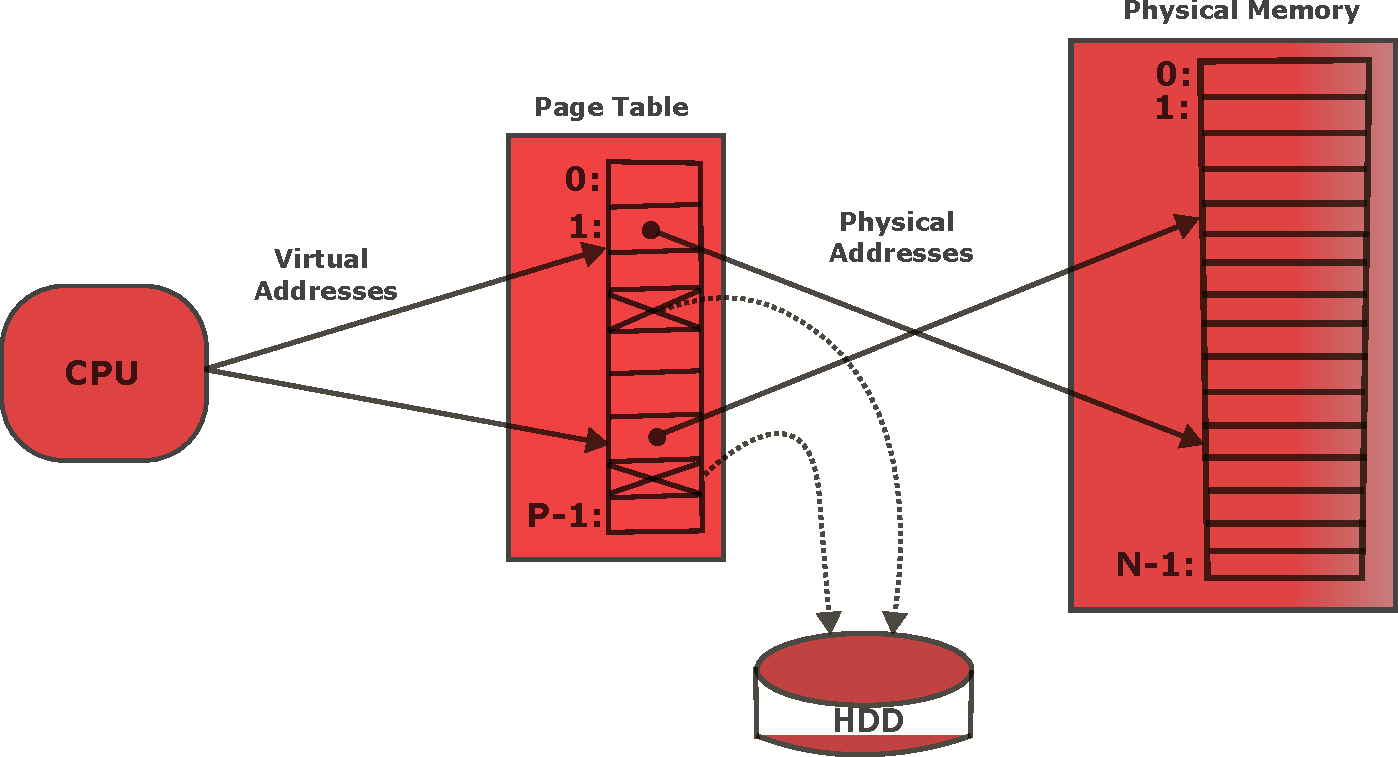
\includegraphics[width=0.85 \linewidth ]{pic/VM.pdf}
	\end{figure}
	\vspace{-0.35cm}
\begin{itemize}
			\item \textbf{Address Translation}: The hardware converts virtual addresses into physical addresses via an OS-managed lookup table (page table).
		\end{itemize}
\end{frame}

\section{\textbf{Address Translation}}

\begin{frame}{\textbf{Address Translation}}
	\begin{figure}
		\centering 
		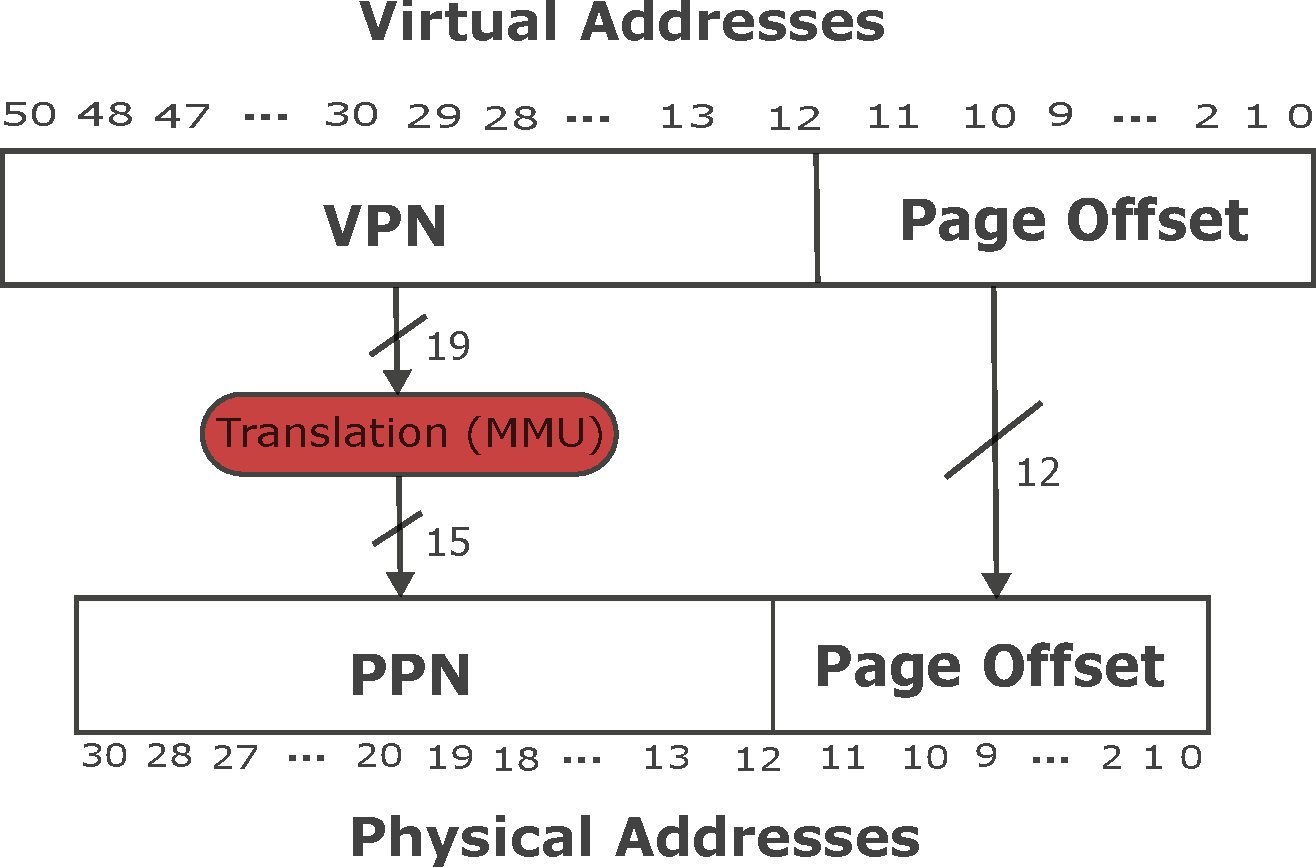
\includegraphics[width=0.8 \linewidth]{pic/translation2.pdf}
	\end{figure}
\end{frame}

\begin{frame}{\textbf{Virtual Memory Example}}
	\begin{itemize}
		\item \textcolor{red}{System}: 
		\begin{itemize}
			\item Virtual Memory capacity: $2$ GB $= 2^{31}$ bytes 
			\item Physical Memory capacity: $128$ MB $= 2^{27}$ bytes
			\item Page size: $4$ KB $= 2^{12}$ bytes 
		\end{itemize}
		
			\item \textcolor{red}{Organisation}: 
		\begin{itemize}
			\item Virtual address: $31$ bits 
			\item Physical address: $27$ bits 
			\item Page offset: $12$ bits
			\item Virtual pages  $= 2^{31} / 2^{12} = \mathbf{2^{19}}$ (VPN = $19$ bits)
			\item Physical pages  $= 2^{27} / 2^{12} = \mathbf{2^{15}}$ (PPN = $15$ bits)
		\end{itemize}
	\end{itemize}
\end{frame}

\begin{frame}[fragile]{\textbf{How Do We translate Addresses?}}
	\begin{itemize}
		\item Page table
		\begin{itemize}
			\item  Has entry for each virtual page
		\end{itemize}
		\item Each page table entry has: 
		\begin{itemize}
			\item Valid bit: whether the virtual page is located in physical memory (if not, it must be fetched from the hard disk)
			\item Physical page number: where the virtual page is located inphysical memory
			 \item (Replacement policy, dirty bits)
		\end{itemize}
	\end{itemize}
\end{frame}

\begin{frame}{\textbf{Page Table Example}}
	\begin{figure}
		\centering 
		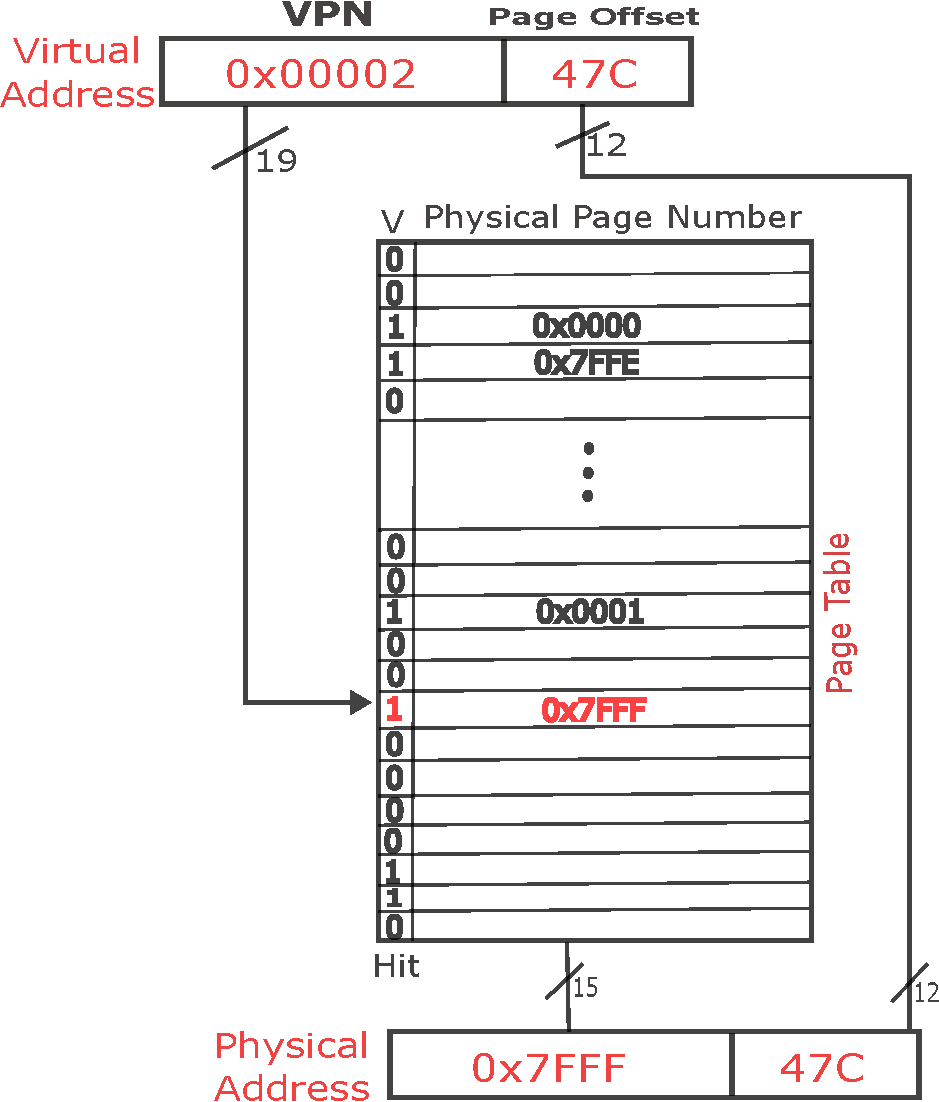
\includegraphics[height=7.7cm, width=0.6 \linewidth]{pic/pageTable3.pdf}
	\end{figure}
\end{frame}


\begin{frame}{\textbf{Page Table Example} (Homework 1)}
	\begin{minipage}{0.5\textwidth}
Consider the PPN on the right. 
	
	\begin{enumerate}
		\item What is the physical address of virtual address \textbf{0x5F20}?
		\item What is the physicaladdress of virtual address \textbf{0x73E0}?
	\end{enumerate}
	\end{minipage}%
	\begin{minipage}{0.5\textwidth}
		\centering
		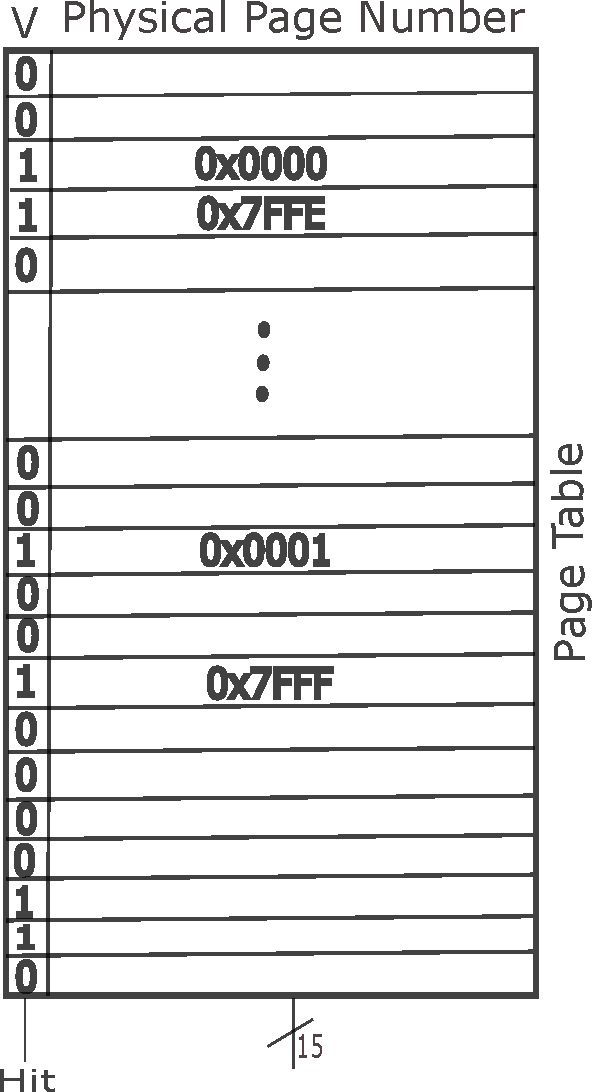
\includegraphics[height=7.6cm, width=0.8 \linewidth]{pic/homework2.pdf}
	\end{minipage}
\end{frame}

\begin{frame}{\textbf{Issues with the Page Table Size}}
	\begin{figure}
		\centering
		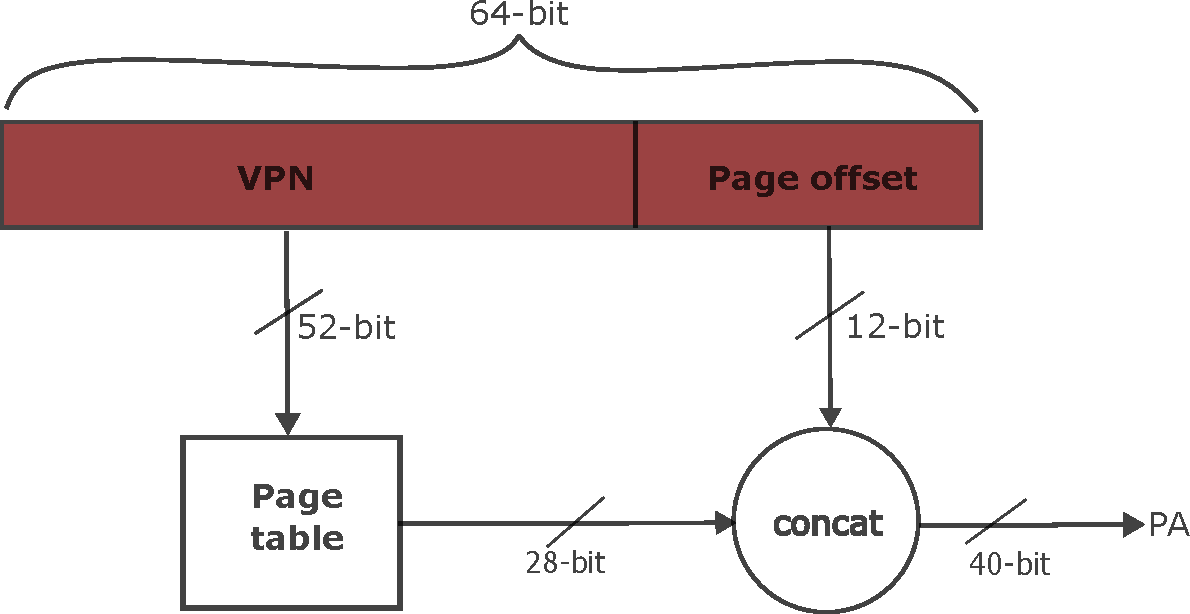
\includegraphics[width=0.8 \linewidth]{pic/page_issue.pdf}
	\end{figure}
	\begin{itemize}
		\item Suppose a $64-$bit VA and a $40-$bit PA, how large is the page table? 
	\end{itemize}
\end{frame}
\begin{frame}{\textbf{Page Table Challenges}}
	\begin{itemize}
		\item Page table accesses have a lot of temporal locality
		\begin{itemize}
			\item  at least part of it needs to be located in physical memory
			\item Data accesses have temporal and spatial locality
			\item Large page size (say 4KB, 8KB, or even 1-2GB), so consecutive loads/stores likely to access same page
		\end{itemize}
		\item Each load/store requires at least two memory accesses:
		
		\begin{enumerate}
			\item one for address translation (page table read)
			\item one to access data with the physical address (after translation)
		\end{enumerate}
		 \item Two memory accesses to service a load/store greatly degrades load/store execution time
		 	\begin{itemize}
		 		\item Unless we are clever…31
		 	\end{itemize}
	\end{itemize}
\end{frame}
\section{\textbf{Translation Lookaside Buffer (TLB)}}

\begin{frame}{\textbf{Translation Lookaside Buffer (TLB)}}
 \textbf{Idea}: Cache the page table entries (PTEs) in a hardwarestructure in the processor
 
\vspace{0.4cm}
\textbf{Advantages}:
		\begin{itemize}
			\item Small cache of most recently used translations (PTEs)
			\item Reduces number of memory accesses required for mostloads/stores to only one
			\item High associativity
			\item Typically 16 - 512 entries
			\item > 95-99 \% hit rates typical (depends on workload)
		\end{itemize}
\end{frame}
%\begin{frame}{\textbf{Example Two-Entry TLB}}
%	
%	\begin{figure}
%		\centering 
%		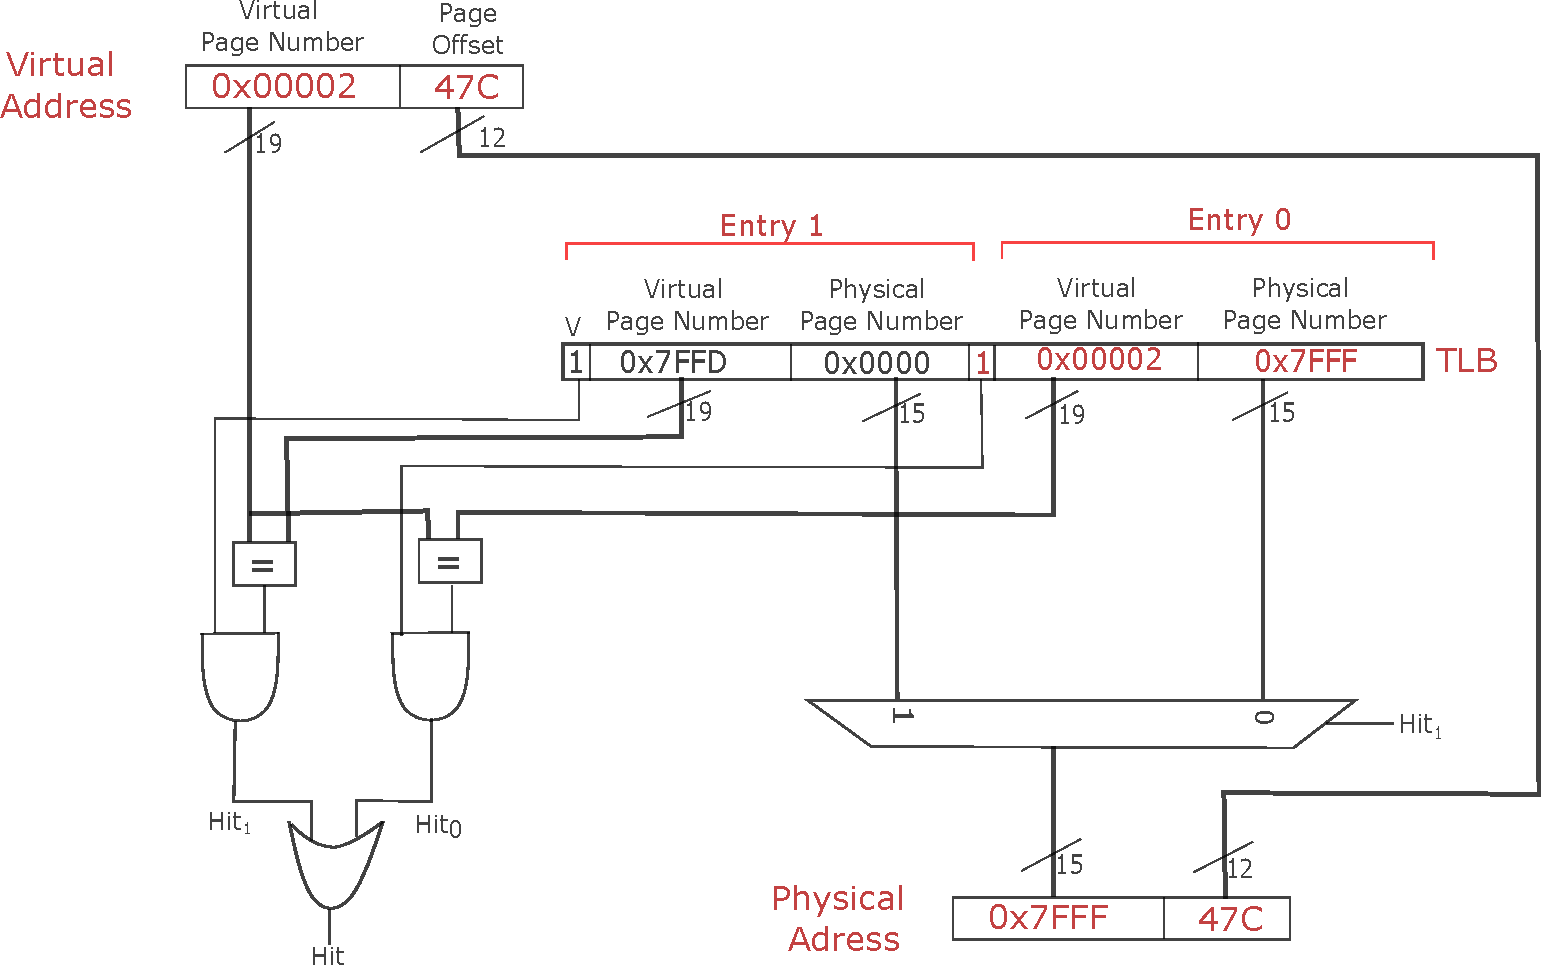
\includegraphics[width= 0.85\linewidth]{pic/TLB.pdf}
%	\end{figure}
%\end{frame}

\begin{frame}[fragile]{\textbf{Multiprossessing and Address Translation}}
	\textbf{Memory Protection}
		\begin{itemize}
			\item Multiple programs (processes) run at once
			\begin{itemize}
				\item Each process has its own page table
				\item Each process can use entire virtual address space without worrying about where other programs are
			\end{itemize}
			\item A process can only access physical pages mapped in its page table---cannot overwrite memory of another process
			\begin{itemize}
				\item Provides protection and isolation between processes
				\item Enables access control mechanisms per page
			\end{itemize}
		\end{itemize}
	
\textbf{Page Table is per Process}\\
		\begin{itemize}
			\item Each process has its own virtual address space
			\begin{itemize}
				\item Full address space for each program
				\item Simplifies memory allocation, sharing, linking and loading. 
			\end{itemize}
		\end{itemize}
\end{frame}
			
\section{\textbf{Takeaway}}

\begin{frame}[fragile]{\textbf{Key Takeaways}}
	\begin{itemize}
		\item \textbf{Virtual memory} gives each process a large, private address space.
		\item The \textbf{OS and hardware} jointly translate virtual addresses to physical addresses.
		\item \textbf{Page tables} do the mapping; \textbf{TLB} makes it fast.
		\item Per-process page tables enforce \textbf{memory protection}.
		\item A subset of virtual pages are located in physical memory
	\end{itemize}
\end{frame}

\section{\textbf{Practical Exercises}}
\begin{frame}{Practical Exercises}
	\begin{enumerate}
		\item Consider a virtual address space of $64$ pages of $1024$ words each, mapped onto a physical memory of $32$ frames.
		\begin{enumerate}
			\item [a. ] How many bits are there in the logical address? 
			\item[b. ] How many bits are there in the physical address?
		\end{enumerate}
		\item Assuming a 1-KB page size, what are the page numbers and offsets for the following address references (provided as decimal numbers): 
		\begin{enumerate}
			\item[a. ] $3085$
			\item[b. ] $42095$
			\item [c. ] $2000001$
		\end{enumerate}
		
		\item Suppose process $X$ and process $Y$ both have a virtual page 2.
		\begin{itemize}
			\item [a. ] $X$'s page $2$ maps to frame $13$; $Y$'s page $2$ to frame $21$.
			\item [b.] If $Y$ reads from virtual address \texttt{0x2004} (4KB pages), what physical address in RAM is accessed?
		\end{itemize}
	\end{enumerate}
	
	%\vspace{0.5cm}
	%\noindent\textbf{Solution to Challenge:} For 4KB pages, frame 21 starts at \texttt{21*4096 = 0x21000}; add offset 0x004: \texttt{0x21004}.
	
\end{frame}

\section{\textbf{What Next?}}
	
	\begin{frame}{What next?}
		\begin{block}{}
			\vspace{0.1cm}
			Page Fault and Page replacement, Structure of Page tables.
		\end{block}
	\end{frame}
	\begin{frame}{Beyond Virtual Memory}
		\begin{enumerate}
			\item Cache Memory (Cache of Level 1, 2, 3 and 4)
			\item Swapping Memory 
			\item IA-32 and x86-64 Memory Architecture
		\end{enumerate}
		\begin{block}{\textbf{Some Important Materials}}
			\begin{itemize}
				\item Operating System Concepts, Abraham Silbershatz, Peter Baer G. and Greg Gagne, Tenth Edition, 2018.
				\item \href{https://www.youtube.com/watch?v=3gRBOqf9rRY}{Youtube Course on Virtual Memory by  Prof. Onur Mutlu, ETH Zürich}
				\item \href{https://github.com/lemerleau/VMAT.git}{Code and Course Material}
			\end{itemize}
		\end{block}
	\end{frame}
	
	
\end{document}
